\documentclass[11pt]{article}
\usepackage[utf8]{inputenc}

% PACKAGES %%%%%%%%%%%%%%%%%%%%%%%%%%%%%%%%%%%%%%%%%%%%%%%%%%%%%%%%%%%%%%%%%%%%%

\usepackage{amsmath,amssymb}
\usepackage[T1]{fontenc} % font encoding
\usepackage{graphicx} % for figures
\usepackage{float} % for figures
\usepackage{indentfirst} % indent first paragraph of section
\usepackage{soul,xcolor} % for colors
\usepackage{xkcdcolors} % colors from XKCD color survey
\usepackage{mathtools} % for boxed equations within \align
\usepackage{sectsty} % adjust section headers
\usepackage{fancyhdr} % page headers
\usepackage{titling} % reference title,author,date (in fancyhdr page header)
\usepackage{breqn} % automatically line wrap long Eqs.
\usepackage{pdfpages} % for \includepdf
\usepackage{pdflscape} % landscape 
\usepackage{mdframed} % for framed environment
\usepackage{minted} % for syntax-highlighted code blocks
\usepackage{inconsolata} % better monospace font
\usepackage[letterpaper, total={6.5in, 9in}]{geometry} % set paper and margin size
\usepackage{empheq} % multiline boxed equations, etc.
\usepackage{hyperref} % hyperlinked references?
\usepackage{dsfont}	% gives you \mathds{} font
\usepackage{multirow} % merged cells in tabular
% \usepackage{enumerate} % custom enumerate numbering (or lettering in this case)
\usepackage[shortlabels]{enumitem} % more enumerate options
\usepackage{svg} % use inkscape to import svgs
\usepackage{bm} % bold symbols
\usepackage[parfill]{parskip} % replace indentation with paragraph spacing
\usepackage{nicematrix} % extended matrix features
\usepackage{nomencl} % nomenclature section
\usepackage{etoolbox} % nomenclature subsections among other things

% FORMATTING %%%%%%%%%%%%%%%%%%%%%%%%%%%%%%%%%%%%%%%%%%%%%%%%%%%%%%%%%%%%%%%%%%%

% add page headers
\pagestyle{fancy}
\fancyhf{}
\fancyhead[LE,LO]{\thetitle}
\fancyhead[RE,RO]{\theauthor}
\fancyfoot[CE,CO]{\thepage}

% adjust section header font size
\sectionfont{\fontsize{20}{15}\selectfont}
\subsectionfont{\fontsize{14}{15}\selectfont}


% LISTINGS %%%%%%%%%%%%%%%%%%%%%%%%%%%%%%%%%%%%%%%%%%%%%%%%%%%%%%%%%%%%%%%%%%%%%

% set code block formats
\definecolor{code_bg}{gray}{0.95}
\definecolor{console_bg}{gray}{1.00}
\setminted{
    bgcolor=code_bg,
    fontsize=\small,
    linenos,
    autogobble}
\setminted[python-console]{
    bgcolor=console_bg,
    linenos=false
    }

% NOMENCLATURE TABLE %%%%%%%%%%%%%%%%%%%%%%%%%%%%%%%%%%%%%%%%%%%%%%%%%%%%%%%%%%%
\renewcommand\nomgroup[1]{%
  \item[\bfseries
  \ifstrequal{#1}{A}{Acronyms}{%
  \ifstrequal{#1}{S}{Symbols}{%
  \ifstrequal{#1}{N}{Notation}{}}}%
]}

% MATH MACROS %%%%%%%%%%%%%%%%%%%%%%%%%%%%%%%%%%%%%%%%%%%%%%%%%%%%%%%%%%%%%%%%%%

% real and imaginary components
\renewcommand{\Re}{\operatorname{Re}}
\renewcommand{\Im}{\operatorname{Im}}

% Fourier transforms
% \newcommand\fourier[1]{\frac{1}{\sqrt{2\pi}} \int_{-\infty}^\infty #1 e^{-i\omega x} \textrm{d}x}
% \newcommand\inverseFourier[1]{\frac{1}{\sqrt{2\pi}} \int_{-\infty}^\infty #1 e^{i\omega x} \textrm{d}\omega}
\newcommand\fourier[1]{\int_{-\infty}^\infty #1 e^{-i\omega x} \textrm{d}x}
\newcommand\inverseFourier[1]{\frac{1}{2\pi} \int_{-\infty}^\infty #1 e^{i\omega x} \textrm{d}\omega}

% derivatives
\newcommand{\ppf}[2]{\frac{\partial #1}{\partial #2}}
\newcommand{\pppf}[3]{\frac{\partial^2 #1}{\partial #2 \partial #3}}
\newcommand{\ddf}[2]{\frac{\text{d} #1}{\text{d} #2}}
\newcommand{\DDf}[2]{\frac{\text{D} #1}{\text{D} #2}}

% norms
\newcommand\norm[1]{\left\lVert#1\right\rVert}

% statistical operators
\newcommand{\prob}{\operatorname{P}}
\newcommand{\expectation}{\operatorname{E}}
\newcommand{\variance}{\operatorname{Var}}
\newcommand{\stddev}{\operatorname{SD}}

% statistical distributions
\newcommand{\bernoulli}{\operatorname{Bernoulli}}
\newcommand{\binomial}{\operatorname{Binomial}}
\newcommand{\poisson}{\operatorname{Poisson}}
\newcommand{\normal}{\operatorname{Normal}}

% hyperbolic trig inverse functions
\DeclareMathOperator{\sech}{sech}
\DeclareMathOperator{\csch}{csch}
\DeclareMathOperator{\arcsec}{arcsec}
\DeclareMathOperator{\arccot}{arcCot}
\DeclareMathOperator{\arccsc}{arcCsc}
\DeclareMathOperator{\arccosh}{arcCosh}
\DeclareMathOperator{\arcsinh}{arcsinh}
\DeclareMathOperator{\arctanh}{arctanh}
\DeclareMathOperator{\arcsech}{arcsech}
\DeclareMathOperator{\arccsch}{arcCsch}
\DeclareMathOperator{\arccoth}{arcCoth} 

% highlighting in math mode
\newcommand{\mathhl}[1]{\colorbox{yellow}{$\displaystyle #1$}}

% COMMONLY USED COPYPASTAS %%%%%%%%%%%%%%%%%%%%%%%%%%%%%%%%%%%%%%%%%%%%%%%%%%%%%

%% CODE BLOCK

% \begin{listing}[H]
%     \caption{Code and output}
%     \label{lst1}
%     \begin{minted}{python}
%         import numpy as np
%         A = np.array([1, 2, 3])
%         print('Hello World')
%     \end{minted}
%     \begin{minted}{python-console}
%         Hello World
%     \end{minted}
% \end{listing}

% \inputminted{python}{helloworld.py}



%% MULTIPLE EQUATIONS BOXED

% \begin{empheq}[box=\fbox]{align}
% \end{empheq}



%% ENUMERTATE WITH a) instead of 1.

% \begin{enumerate}[label=\alph*)]
% \end{enumerate}



%% SET CURRENT SUBHEADER NUMBER

% \setcounter{subsection}{1}
% 'Problem' sections
\renewcommand{\thesection}{\arabic{section}}
\renewcommand{\thesubsection}{\arabic{section}.\alph{subsection}}
\renewcommand{\thesubsubsection}{\arabic{section}.\alph{subsection}.\roman{subsubsection}}
% \renewcommand{\thesubsection}{\arabic{subsection}}


\title{ENGR 520 Homework 2}
\author{Anthony Su}
\date{April 29, 2025}

\begin{document}
\thispagestyle{plain}
\maketitle


\textbf{Collaboration statement:} I did not collaborate with others on this assignment. I utilized large language models for code debugging.


%%%%%%%%%%%%%%%%%%%%%%%%%%%%%%%%%%%%%%%%%%%%%%%%%%%%%%%%%%%%%%%%%%%%%%%%%%%%%%%%
% 1. Dynamic Mode Decomposition
%%%%%%%%%%%%%%%%%%%%%%%%%%%%%%%%%%%%%%%%%%%%%%%%%%%%%%%%%%%%%%%%%%%%%%%%%%%%%%%%
\section{Dynamic Mode Decomposition}

\subsection{Full Clean Data} % a -----------------------------------------------

The dynamic mode decomposition (DMD) was performed on the vorticity of flow past a cylinder. A snapshot visualizing the flow field is shown in Figure \ref{fig1a1}. The first 21 eigenvalues of this DMD solution are shown in Figure \ref{fig1a2}.

\begin{figure}[H]
    \centering
    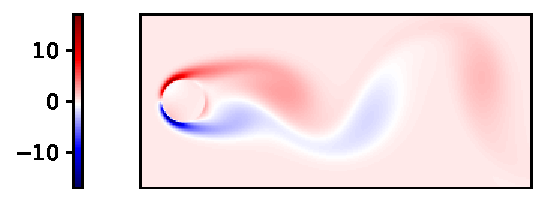
\includegraphics[width=3.5in]{fig1a_snapshot.pdf}
    \caption{Snapshot of clean data}
    \label{fig1a1}
\end{figure}

\begin{figure}[H]
    \centering
    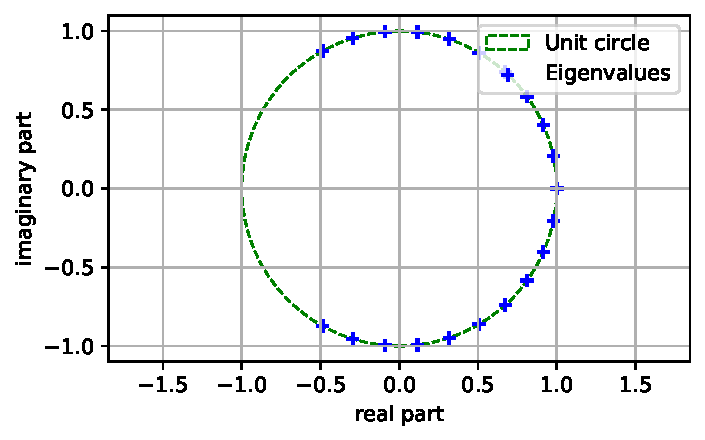
\includegraphics[width=4in]{fig1a_eigs.pdf}
    \caption{Eigenvalues of clean data}
    \label{fig1a2}
\end{figure}

For a discrete-time system, eigenvalues on the unit circle represent purely oscillatory modes (with no damping/dissipation). This is physically equivalent to energy conservation.

\subsection{Full Noisy Data} % b -----------------------------------------------

Noise of three different magnitudes was added to the vorticity data and the DMD was performed again for each magnitude of noise. Snapshots visualizing the impact of noise are shown in Figures \ref{fig1b1}, \ref{fig1b2}, and \ref{fig1b3}. The first 21 eigenvalues of these DMD solutions are shown in Figures \ref{fig1b4}, \ref{fig1b5}, and \ref{fig1b6}.

The DMD eigenvalues of the noisy data are misleading because they do not lie on the unit circle, but rather inside of it. This implies energy dissipation, which is not actually occurring in the underlying data; this is an artifact of the added noise. The more significant first few modes are less sensitive to noise than the less significant later modes.

\begin{figure}[H]
    \centering
    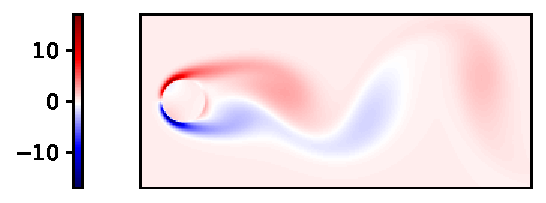
\includegraphics[width=3.5in]{fig1b_snapshot_1.pdf}
    \caption{Snapshot of 1\% noisy data}
    \label{fig1b1}
\end{figure}

\begin{figure}[H]
    \centering
    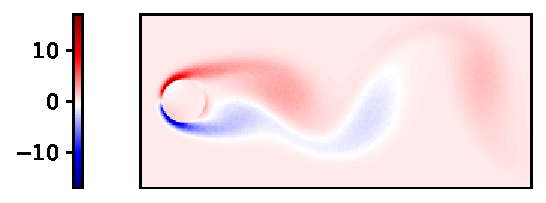
\includegraphics[width=3.5in]{fig1b_snapshot_2.pdf}
    \caption{Snapshot of 10\% noisy data}
    \label{fig1b2}
\end{figure}

\begin{figure}[H]
    \centering
    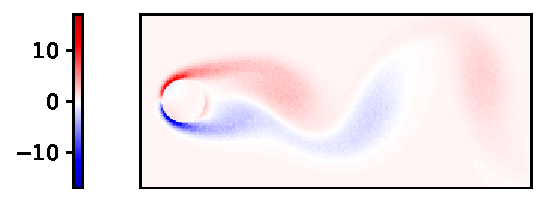
\includegraphics[width=3.5in]{fig1b_snapshot_3.pdf}
    \caption{Snapshot of 20\% noisy data}
    \label{fig1b3}
\end{figure}

\begin{figure}[H]
    \centering
    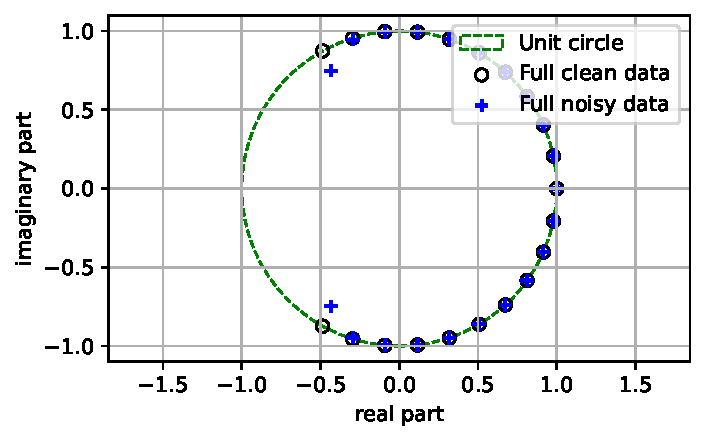
\includegraphics[width=4in]{fig1b_eigs_1.pdf}
    \caption{Eigenvalues of 1\% noisy data}
    \label{fig1b4}
\end{figure}

\begin{figure}[H]
    \centering
    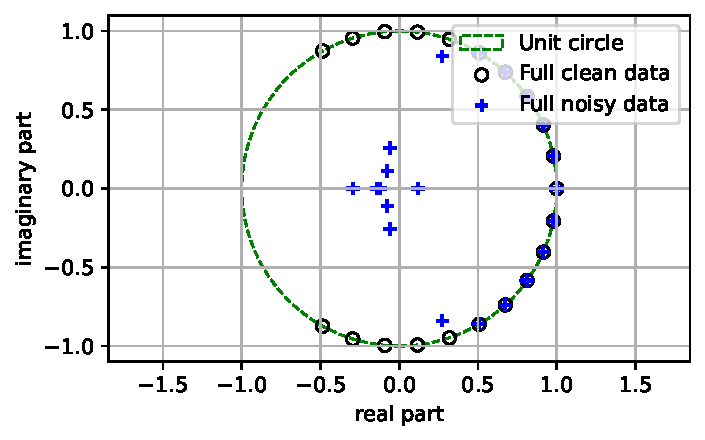
\includegraphics[width=4in]{fig1b_eigs_2.pdf}
    \caption{Eigenvalues of 10\% noisy data}
    \label{fig1b5}
\end{figure}

\begin{figure}[H]
    \centering
    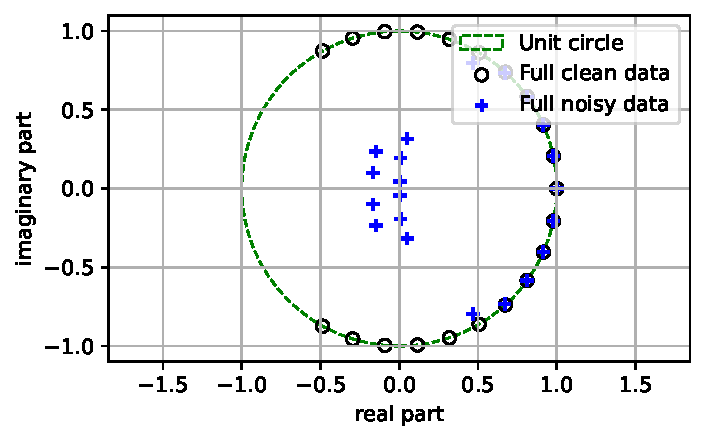
\includegraphics[width=4in]{fig1b_eigs_3.pdf}
    \caption{Eigenvalues of 20\% noisy data}
    \label{fig1b6}
\end{figure}

\subsection{Subset of Clean Data} % c ------------------------------------------

The vorticity data was truncated so that its length was 75\% of the vortex shedding period and DMD was performed on this truncated data.

The DMD eigenvalues of the truncated data also lie within the unit circle, falsely implying dissipation. Unlike for the noisy data, the sensitivity of the various modes to this source of error is more evenly distributed across the modes (but the higher modes are still more sensitive).

\begin{figure}[H]
    \centering
    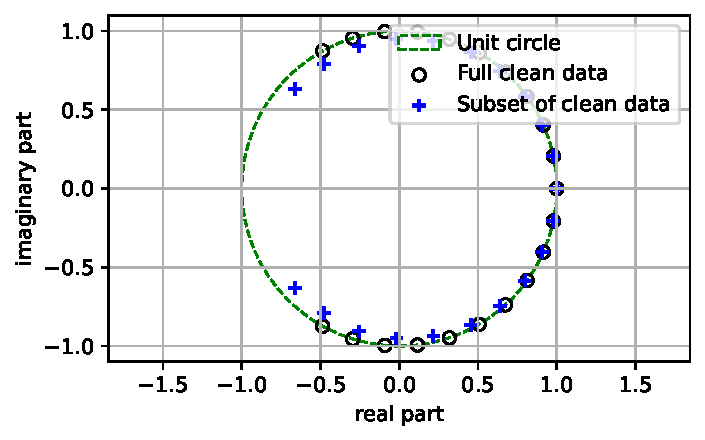
\includegraphics[width=4in]{fig1c_eigs.pdf}
    \caption{Eigenvalues of clean data subset}
    \label{fig1c1}
\end{figure}


\subsection*{Physics-Informed Dynamic Mode Decomposition}

In this flow field, physics that would be useful to include would be:
\begin{itemize}
    \item periodicity (energy conservation)
    \item shift-invariance
    \item mass continuity
\end{itemize}


%%%%%%%%%%%%%%%%%%%%%%%%%%%%%%%%%%%%%%%%%%%%%%%%%%%%%%%%%%%%%%%%%%%%%%%%%%%%%%%%
% 2. Physics-Informed Neural Networks
%%%%%%%%%%%%%%%%%%%%%%%%%%%%%%%%%%%%%%%%%%%%%%%%%%%%%%%%%%%%%%%%%%%%%%%%%%%%%%%%
\section{Physics-Informed Neural Networks}

\subsection{Loss Function} % a -------------------------------------------------

The physics-informed loss function $L$ is defined as:
\begin{align*}
    L(\theta) &=
    \operatorname{MSE}\left(\hat{u}, u\right)
    + \operatorname{MSE}\left(\hat{v}, v\right)
    + \operatorname{MSE}\left(\ppf{\hat{u}}{x} + \ppf{\hat{v}}{y}, 0\right)
\end{align*}
where
\begin{itemize}
    \item $\operatorname{MSE}(a, b) = \frac{1}{n} \sum_{i=1}^n (b-a)^2$
    \item $\lambda$ is the weight of the physics loss term
    \item $n$ is the number of training data points
    \item $m$ is the number of virtual points (for computing physics error)
    \item $\boldsymbol{u}$ is the true velocity vector
    \item $\hat{\boldsymbol{u}}$ is the estimated velocity vector computed by the model $f_\theta(\boldsymbol{x})$
\end{itemize}
The first two terms of $L$ are the mean-squared error (MSE) of the model $f_\theta$ across all $n$ training data points. The third term of $L$ is the mean-squared \textit{physics} error (flow divergence) of $f_\theta$ across all $m$ virtual points.

\subsection{Full Data} % b -------------------------------------------------

Interpolation outperforms my PINN with the full data.
\begin{table}[H]
    \centering
    \caption{Full data model performance}
    \begin{tabular}{|c|c|c|}
        \hline
        flow & method & data loss \\
        \hline
        \hline
        linear potential vortex & neural network & 6.478e-05 \\
        linear potential vortex & linear interpolation & 4.545e-33 \\
        Taylor-Green potential vortex & neural network & 1.164e+00 \\
        Taylor-Green potential vortex & linear interpolation & 1.123e+00 \\
        \hline
    \end{tabular}
    \label{tab1b}
\end{table}

\subsection{Half Data} % c -------------------------------------------------

My PINN should outperform linear interpolation when trained on half of the data and tested on the other half. I think there's an issue with my linear potential vortex interpolation implementation.

\begin{table}[H]
    \centering
    \caption{Half data model extrapolation performance}
    \begin{tabular}{|c|c|c|}
        \hline
        flow & method & data loss \\
        \hline
        \hline
        linear potential vortex & PINN & 1.760e-01 \\
        linear potential vortex & linear interpolation & 1.573e-31 \\
        Taylor-Green potential vortex & PINN & 1.101e+00 \\
        Taylor-Green potential vortex & linear interpolation & 2.180e+00 \\
        \hline
    \end{tabular}
    \label{tab1c}
\end{table}

\subsection{Symmetry} % d ------------------------------------------------------

The symmetry can be enforced in the linear potential vortex with the following loss term:
\begin{align*}
    \operatorname{MSE}\left(\hat{u}, -\hat{u}_r\right) + \operatorname{MSE}\left(\hat{v}, -\hat{v}_r\right)
\end{align*}
and in the Taylor-Green potential vortex with the following loss term:
\begin{align*}
    \operatorname{MSE}\left(\hat{u}, 1-\hat{u}_m\right) + \operatorname{MSE}\left(\hat{v}, \hat{v}_m\right)
\end{align*}
where
\begin{itemize}
    \item $\left(\hat{u}, \hat{v}\right) = f_\theta(x, y)$
    \item $\left(\hat{u}_r, \hat{v}_r\right) = f_\theta(-x, -y)$
    \item $\left(\hat{u}_m, \hat{v}_m\right) = f_\theta(-x, y)$
\end{itemize}

My PINN with symmetry loss should outperform linear interpolation when trained on half of the data and tested on the other half. I think there's an issue with my linear potential vortex interpolation implementation.

Enforcing symmtetry leads to improvement over the PINN without symmetry for the linear potential vortex.

\begin{table}[H]
    \centering
    \caption{Half data model extrapolation performance}
    \begin{tabular}{|c|c|c|}
        \hline
        flow & method & data loss \\
        \hline
        \hline
        linear potential vortex & PINN with symmetry & 2.268e-04 \\
        linear potential vortex & linear interpolation & 1.573e-31 \\
        Taylor-Green potential vortex & PINN with symmetry & 1.068e+00 \\
        Taylor-Green potential vortex & linear interpolation & 2.180e+00 \\
        \hline
    \end{tabular}
    \label{tab1d}
\end{table}


\section*{Code Appendix}

Note that code for Section 2.a was modified and re-run for Section 2.b and similarly for Section 2.c, so only code for Section 2.c is shown.

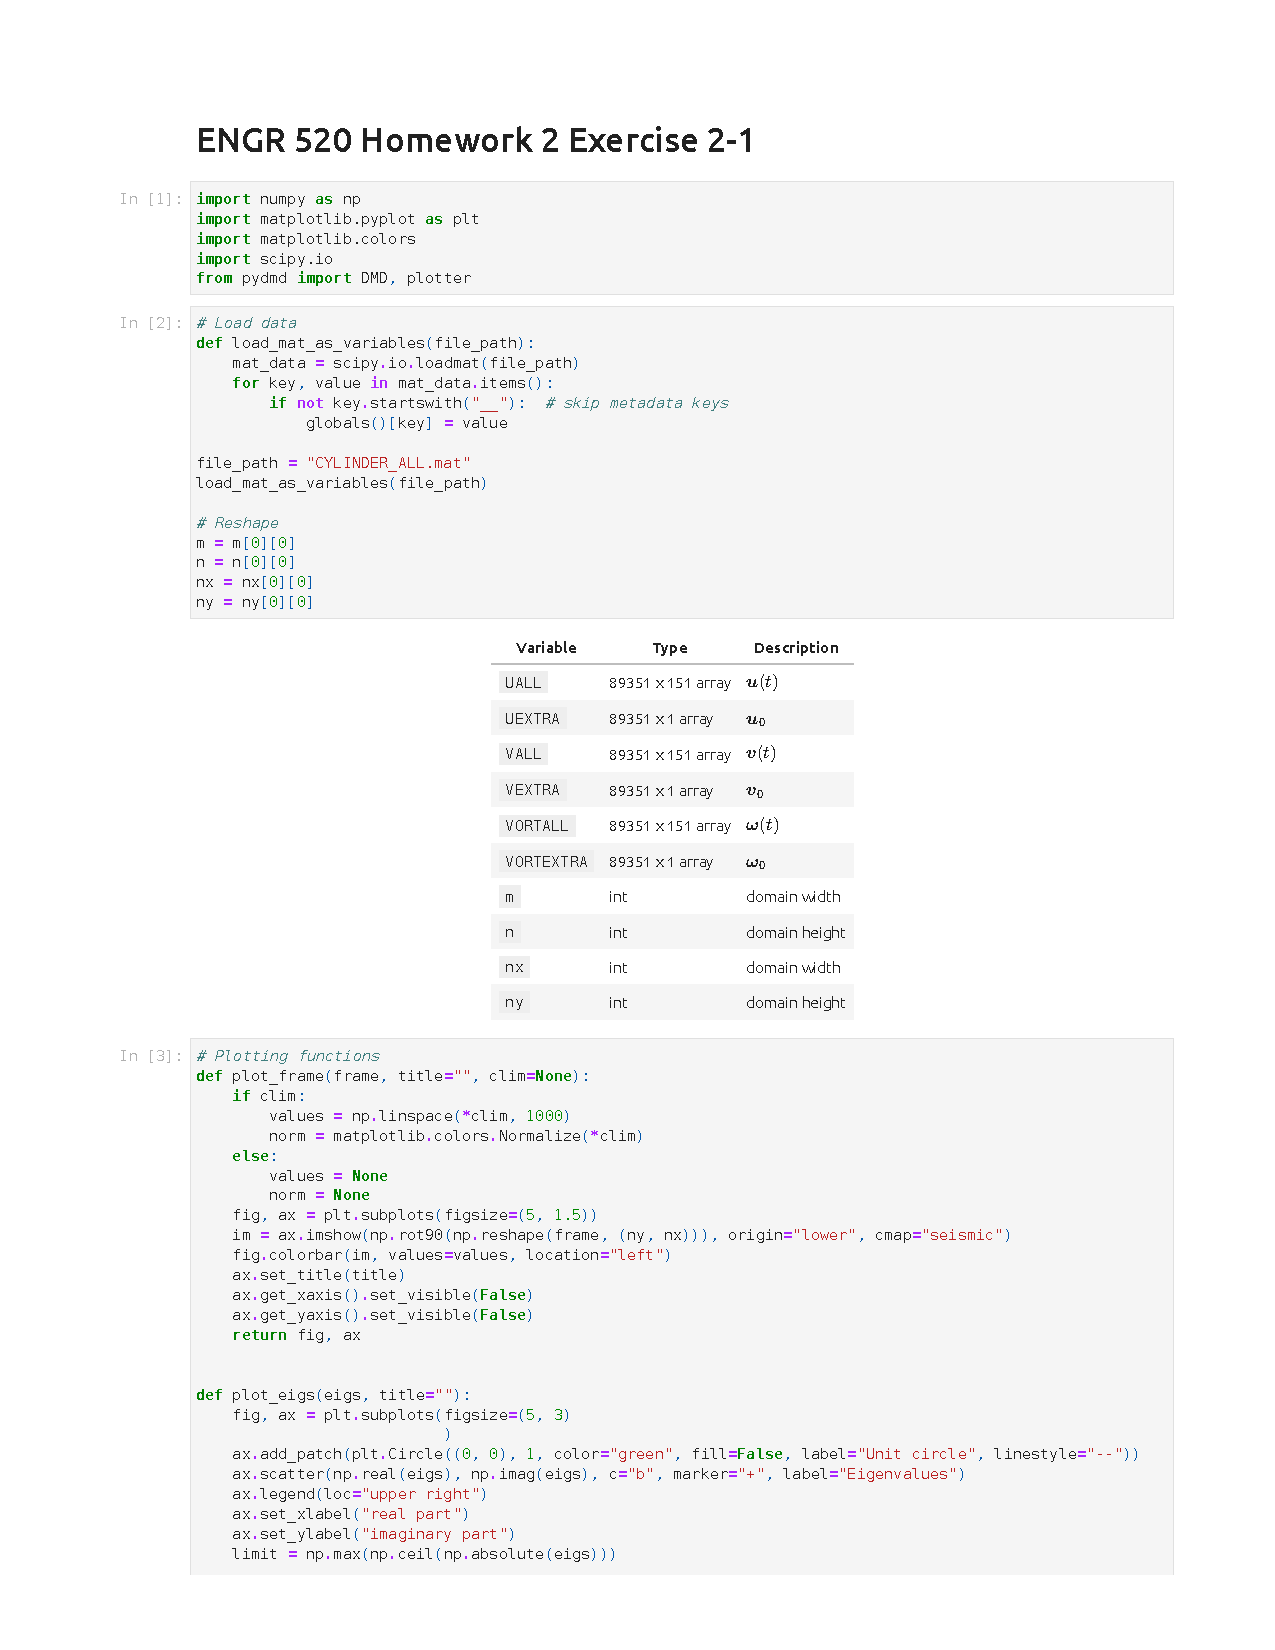
\includepdf[pages=-]{hw2p1nb.pdf}
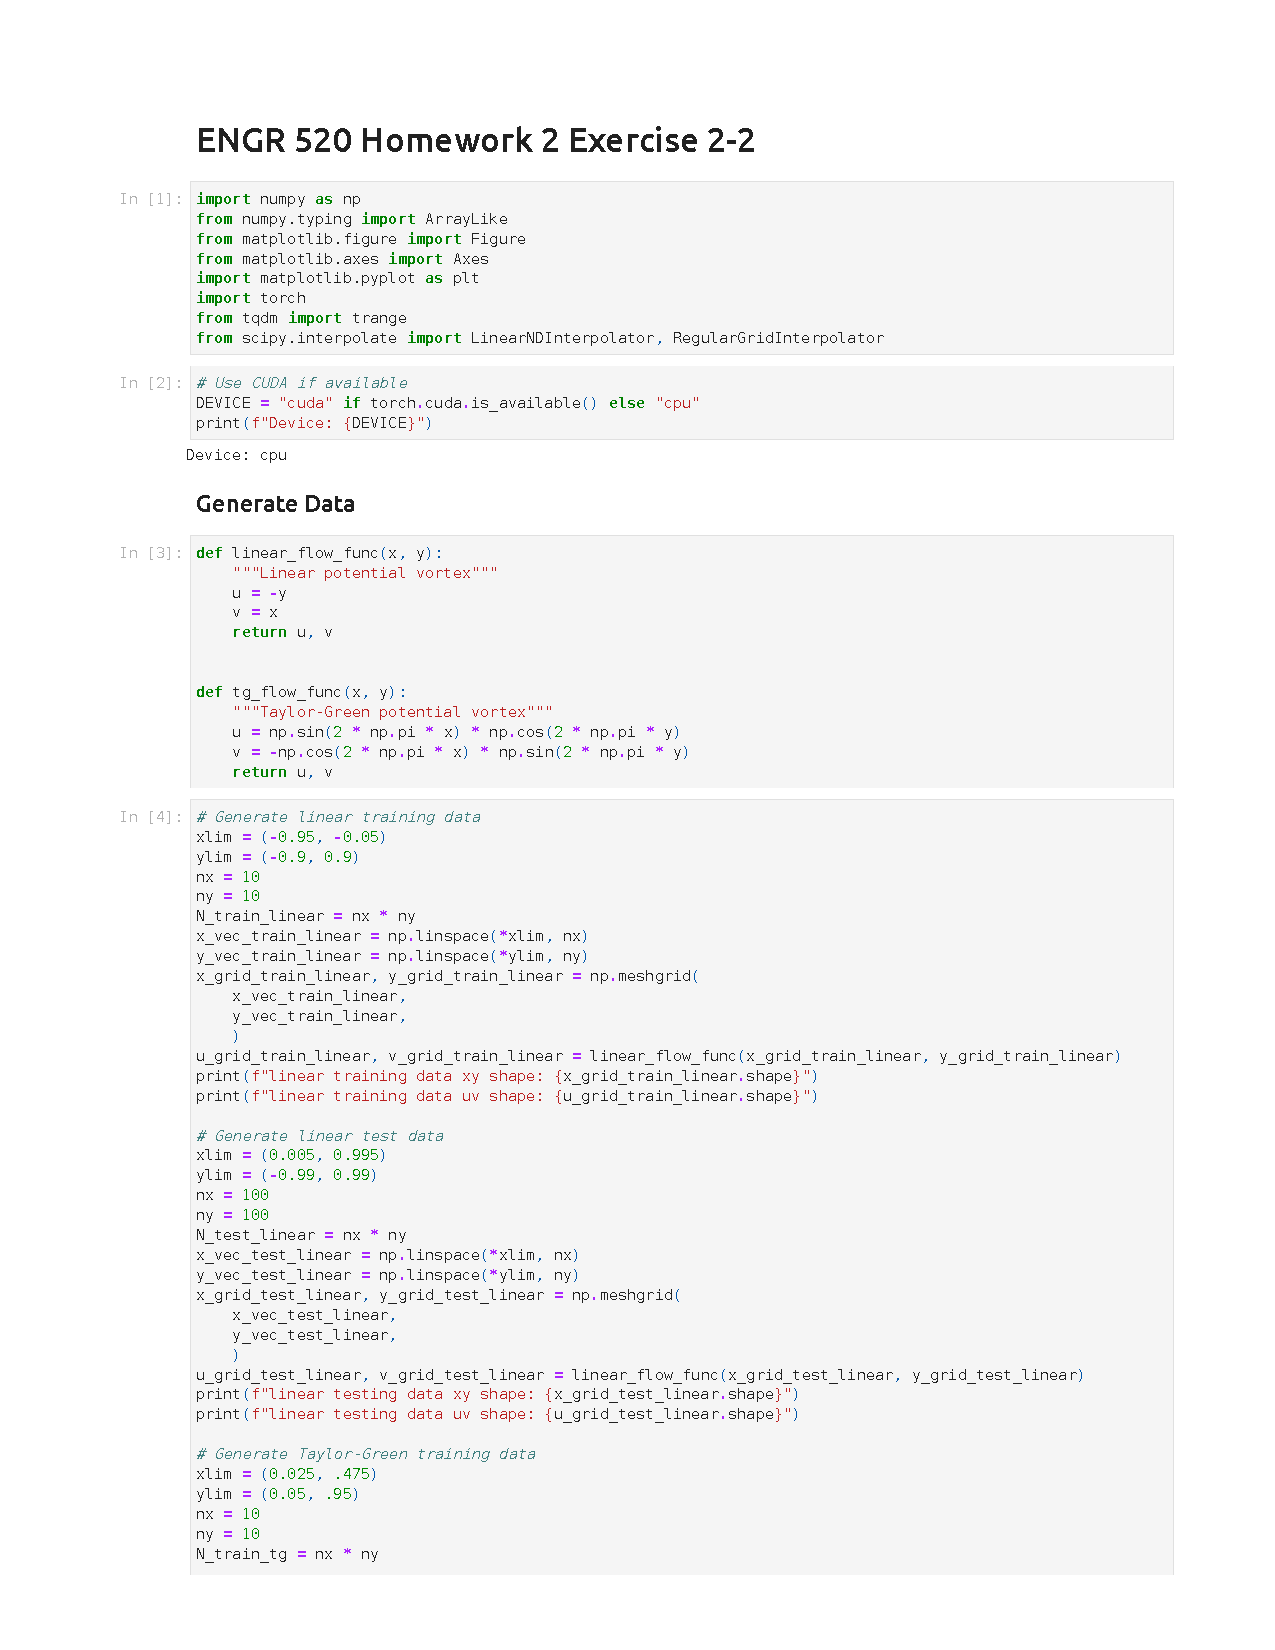
\includepdf[pages=-]{hw2p2nb.pdf}

\end{document}